%% BioMed_Central_Tex_Template_v1.06
%%                                      %
%  bmc_article.tex            ver: 1.06 %
%                                       %

%%IMPORTANT: do not delete the first line of this template

%%%%%%%%%%%%%%%%%%%%%%%%%%%%%%%%%%%%%%%%%
%%                                     %%
%%  LaTeX template for BioVis 2014  %%
%%      article submissions     %%
%%          adapted from BMC    %%
%%          <8 Jan 2014>              %%
%% Liz Marai (g.elisabeta.marai@gmail.com) %%
%%                                     %%
%%%%%%%%%%%%%%%%%%%%%%%%%%%%%%%%%%%%%%%%%


%%%%%%%%%%%%%%%%%%%%%%%%%%%%%%%%%%%%%%%%%%%%%%%%%%%%%%%%%%%%%%%%%%%%%
%%                                                                 %%
%%%%%%%%%%%%%%%%%%%%%%%%%%%%%%%%%%%%%%%%%%%%%%%%%%%%%%%%%%%%%%%%%%%%%

%%% additional documentclass options:
%  [doublespacing]
%  [linenumbers]   - put the line numbers on margins

%%% loading packages, author definitions

\documentclass[twocolumn]{bmcart}% uncomment this for twocolumn layout 



%%% Load packages
%\usepackage{amsthm,amsmath}
%\RequirePackage{natbib}
%\RequirePackage{hyperref}
\usepackage[utf8]{inputenc} %unicode support
%\usepackage[applemac]{inputenc} %applemac support if unicode package fails
%\usepackage[latin1]{inputenc} %UNIX support if unicode package fails
\usepackage{graphicx}
\usepackage{color}
\usepackage[textsize=small,colorinlistoftodos]{todonotes}
\usepackage{algorithm}
\usepackage{algorithmicx}
\usepackage{algpseudocode}
\usepackage{xspace}

%%%%%%%%%%%%%%%%%%%%%%%%%%%%%%%%%%%%%%%%%%%%%%%%%
%%                                             %%
%%  If you wish to display your graphics for   %%
%%  your own use using includegraphic or       %%
%%  includegraphics, then comment out the      %%
%%  following two lines of code.               %%
%%%%%%%%%%%%%%%%%%%%%%%%%%%%%%%%%%%%%%%%%%%%%%%%%


%\def\includegraphic{}
%\def\includegraphics{}



%%% Put your definitions there:
\startlocaldefs
\endlocaldefs


% Defines usefull commands.
\newcommand{\ie}{i.e.,~}
\newcommand{\eg}{e.g.,~}

\algrenewcommand\algorithmicrequire{\textbf{Input:}}
\algrenewcommand\algorithmicensure{\textbf{Output:}}
\algnewcommand\And{\textbf{and}\xspace}
\algnewcommand\Or{\textbf{or}\xspace}

%%% Begin ...
\begin{document}

%%% Start of article front matter
\begin{frontmatter}

\begin{fmbox}
\dochead{Research}

%%%%%%%%%%%%%%%%%%%%%%%%%%%%%%%%%%%%%%%%%%%%%%
%%                                          %%
%% Enter the title of your article here     %%
%%                                          %%
%%%%%%%%%%%%%%%%%%%%%%%%%%%%%%%%%%%%%%%%%%%%%%

\title{Interactive Exploration of Ligand Movements through Multiscale Temporal Tunnels}

%%%%%%%%%%%%%%%%%%%%%%%%%%%%%%%%%%%%%%%%%%%%%%
%%                                          %%
%% Do not enter the authors here for        %%
%%  a double-blind review. Otherwise        %%
%% specify information, if available,       %%
%% in the form:                             %%
%%   <key>={<id1>,<id2>}                    %%
%%   <key>=                                 %%
%% Comment or delete the keys which are     %%
%% not used. Repeat \author command as much %%
%% as required.                             %%
%%                                          %%
%%%%%%%%%%%%%%%%%%%%%%%%%%%%%%%%%%%%%%%%%%%%%%
\author[
   addressref={aff1},
   email={furmanova@mail.muni.cz}
]{\inits{KF}\fnm{Katar\'{i}na} \snm{Furmanov\'{a}}}
\author[
   addressref={aff1},                   % id's of addresses, e.g. {aff1,aff2}
   email={jaresova@mail.muni.cz}   % email address
]{\inits{MJ}\fnm{Miroslava} \snm{Jare\v{s}ov\'{a}}}
\author[
   addressref={aff1,aff2},                   % id's of addresses, e.g. {aff1,aff2}
   email={xbyska@fi.muni.cz}   % email address
]{\inits{JB}\fnm{Jan} \snm{By\v{s}ka}}
\author[
   addressref={aff1},                   % id's of addresses, e.g. {aff1,aff2}
   email={xjurc@fi.muni.cz}   % email address
]{\inits{AJ}\fnm{Adam} \snm{Jur\v{c}\'{i}k}}
\author[
   addressref={aff2},                   % id's of addresses, e.g. {aff1,aff2}
   email={julius.parulek@uib.no}   % email address
]{\inits{JP}\fnm{J\'{u}lius} \snm{Parulek}}
\author[
   addressref={aff2},                   % id's of addresses, e.g. {aff1,aff2}
   email={Helwig.Hauser@uib.no}   % email address
]{\inits{HH}\fnm{Helwig} \snm{Hauser}}
\author[
   addressref={aff1},                   % id's of addresses, e.g. {aff1,aff2}
   email={kozlikova@fi.muni.cz}   % email address
]{\inits{BK}\fnm{Barbora} \snm{Kozl\'{i}kov\'{a}}}

%%%%%%%%%%%%%%%%%%%%%%%%%%%%%%%%%%%%%%%%%%%%%%
%%                                          %%
%% Enter the authors' addresses here        %%
%%                                          %%
%% Repeat \address commands as much as      %%
%% required.                                %%
%%                                          %%
%%%%%%%%%%%%%%%%%%%%%%%%%%%%%%%%%%%%%%%%%%%%%%

\address[id=aff1]{%                           % unique id
  \orgname{Masaryk University}, % university, etc
  %\postcode{15260}                                % post or zip code
  \city{Brno},                              % city
  \cny{Czech Republic}                                    % country
}
\address[id=aff2]{%                           % unique id
  \orgname{University of Bergen}, % university, etc
%  \street{210 South Bouquet},                     %
  %\postcode{15260}                                % post or zip code
  %\city{Williamsburg},                              % city
  \cny{Norway}                                    % country
}

%%%%%%%%%%%%%%%%%%%%%%%%%%%%%%%%%%%%%%%%%%%%%%
%%                                          %%
%% Enter short notes here                   %%
%%                                          %%
%% Short notes will be after addresses      %%
%% on first page.                           %%
%%                                          %%
%%%%%%%%%%%%%%%%%%%%%%%%%%%%%%%%%%%%%%%%%%%%%%

\begin{artnotes}
%\note{Sample of title note}     % note to the article
%\note[id=n1]{Equal contributor} % note, connected to author
%\note[id=n2]{Equal contributor} % note, connected to author
%\note[id=n3]{Equal contributor} % note, connected to author
%\note[id=n4]{Project leader and equal contributor} % note, connected to author
\end{artnotes}

\end{fmbox}% comment this for two column layout

%%%%%%%%%%%%%%%%%%%%%%%%%%%%%%%%%%%%%%%%%%%%%%
%%                                          %%
%% The Abstract begins here                 %%
%%                                          %%
%% Please refer to the Instructions for     %%
%% authors on http://www.biomedcentral.com  %%
%% and include the section headings         %%
%% accordingly for your article type.       %%
%%                                          %%
%%%%%%%%%%%%%%%%%%%%%%%%%%%%%%%%%%%%%%%%%%%%%%

\begin{abstractbox}

\begin{abstract} % abstract, must be under 350 words
%\parttitle{First part title} %if any
%Text for this section.

\parttitle{Background} TODO BK 

\parttitle{Results} TODO BK 

\parttitle{Conclusions}  TODO BK


%\parttitle{Second part title} %if any
%Text for this section.
\end{abstract}

%%%%%%%%%%%%%%%%%%%%%%%%%%%%%%%%%%%%%%%%%%%%%%
%%                                          %%
%% The keywords begin here                  %%
%%                                          %%
%% Put each keyword in separate \kwd{}.     %%
%%                                          %%
%%%%%%%%%%%%%%%%%%%%%%%%%%%%%%%%%%%%%%%%%%%%%%

\begin{keyword}
\kwd{Molecular Sequence Analysis}
\kwd{Molecular Structural Biology}
\kwd{Computational Proteomics}
\end{keyword}

% MSC classifications codes, if any
%\begin{keyword}[class=AMS]
%\kwd[Primary ]{}
%\kwd{}
%\kwd[; secondary ]{}
%\end{keyword}

\end{abstractbox}
%
%\end{fmbox}% uncomment this for twcolumn layout

\end{frontmatter}

%%%%%%%%%%%%%%%%%%%%%%%%%%%%%%%%%%%%%%%%%%%%%%
%%                                          %%
%% The Main Body begins here                %%
%%                                          %%
%% Please refer to the instructions for     %%
%% authors on:                              %%
%% http://www.biomedcentral.com/info/authors%%
%% and include the section headings         %%
%% accordingly for your article type.       %%
%%                                          %%
%% See the Results and Discussion section   %%
%% for details on how to create sub-sections%%
%%                                          %%
%% use \cite{...} to cite references        %%
%%  \cite{koon} and                         %%
%%  \cite{oreg,khar,zvai,xjon,schn,pond}    %%
%%  \nocite{smith,marg,hunn,advi,koha,mouse}%%
%%                                          %%
%%%%%%%%%%%%%%%%%%%%%%%%%%%%%%%%%%%%%%%%%%%%%%

%%%%%%%%%%%%%%%%%%%%%%%%% start of article main body
% <put your article body there>

%%%%%%%%%%%%%%%%
%% Background %%
%%
\section*{Background}

TODO BK + JP (Intro + RW)

\section*{Method}
\subsection*{Overview + workflow - BK}

\subsection*{Temporal Tunnel - JB}
\label{Sec:TemporalTunnel}
\todo{přehodil jsem sekci, sem, bo si myslím, že ji chceme použít aj v simplifikaci ne? + minimálně bude třeba o ní vědět při definování empy space atributu}

\todo{Nevím jak začít .... chce to asi nějakou motivaci proč vůbec temporal tunnel} 

We define the temporal tunnel as a set of spheres where the number of spheres corresponds to the number of time steps in the simulation.
Additionally, each sphere defines the maximum empty space surrounding the ligand, and as the consequence also contains the ligand, in the given time step {\color{red}(see Figure~\ref{XY})}.

In order to compute such temporal tunnel we can either utilize the pre-computed information about protein tunnels (\eg using CAVER~3.0) or approximate information about the empty space surrounding the ligand manually. 
The first method is more precise but computationally more expensive, while the second approach is faster but {\color{red}can be highly inaccurate} {\color{red}see Section~\ref{XYZ} for experimental comparison)}. 
Nevertheless, in both cases we need to determine a single sphere which will be part of temporal tunnel for each time step.

When using the pre--computed data we basically obtain a set of spheres defining the shape of the tunnel in each time step ({\color{red} see Section/Paper about CAVER}). 
Since we also have a ligand position \todo{někde bude třeba definovat ligand position} in each time step we can utilize the aforementioned information about protein tunnels to determine single tunnel sphere containing the ligand in the given time. 
The whole temporal tunnel then can be build simply by selecting the closest sphere to the ligand which is also wide enough \todo{wide enough není zprogramováné} to enclose fully it in each time step. \todo{ty poslední dvě věty se asi opakují.}

%The closest sphere can be find simply by measuring the distance between the center of mass of ligand and center of each sphere.  

{\color{red} Už nestíhám, ale ta druhá metoda byla popsána v předchozím článku, takže jí z tama můžeme vytáhnout - možná to ještě udělám později, zatím teda takto.}


\subsection*{Trajectory Simplification - AJ}
Including mathematical model.

\begin{algorithm}
  \begin{algorithmic}[1]
	  \Require $T$ --- trajectory, $I$ --- interval
	  \Ensure $T$ --- simplified trajectory
		\Procedure{Simplify}{$T, I$}
			\State \Return $T$ \Comment{Tohle bude zajimave popsat bo je to docela slozite}
		\EndProcedure
  \end{algorithmic}
	\caption{Trajectory simplification}
  \label{alg:simplify}
\end{algorithm}

\begin{algorithm}
  \begin{algorithmic}[1]
	  \Require $T$ --- trajectory, $\nu$ --- complexity neighborhood, $\tau$ --- complexity threshold, $\epsilon$ --- improvement threshold
	  \Ensure $T$ --- simplified trajectory
		\Procedure{AutoSimplify}{$T, \nu, \tau, \epsilon$}
			\Repeat
        \State $c(x) \gets$ \Call{ComputeComplexity}{$T, \nu$}
			  \State $I \gets$ \Call{FindComplexInterval}{$c, \tau$}
			  \State
				\State $\Delta c \gets 0$
			  \If{$I \neq \emptyset$}
				  \State $T \gets$ \Call{Simplify}{$T, I$}
				  \State
					\State $c'(x) \gets c(x)$ \Comment{$c'(x)$ --- previous complexity}
				  \State $c(x) \gets$ \Call{ComputeComplexity}{$T, \nu$}
					\State
					\State $\Delta c \gets \sum_{x \in s(T)}{max(c(x) - c'(x), 0)}$
					\State \Comment{$s(T)$ --- snapshots of $T$}
			  \EndIf
			\Until{$\Delta c > \epsilon$ \Or $I = \emptyset$}
			\State
			\State \Return $T$
		\EndProcedure
  \end{algorithmic}
	\caption{Automatic trajectory simplification}
  \label{alg:auto-simplify}
\end{algorithm}

\subsection*{Derivation of Attributes - JB}

In previous section we have described the simplification of the ligand trajectory. 
On one hand, such approximation helps to easily understand the overall ligand movements. 
On the other hand, it also suppresses vast amount of details that are important for the complete understanding of the ligand movements inside protein.

In order to preserve this information and hence allow the biochemist to explore the ligand behaviour in detail we evaluate various geometrical and chemico-physical attributes of the ligand trajectory on multiple levels. 
These attributes are then communicated to the user in various ways (for more details {\color{red}see Section~\ref{XYZ}}).

Among the most important attributes belongs the "stuckenss" of the ligand in one place, its distance from the active site, direction of its movement, amount of surrounding free space, changes of surrounding amino acids and its properties, and relative movements and rotations of the ligand inside the tunnel. 
In the rest of this section we discuss usefulness and the way how we derive individual attributes them from the original data.    

\begin{itemize}

\item \textbf{Stuckness} is one of the most abstract attributes. Fortunately, it can be easily measured. 
We consider the ligand to be stuck if it oscillates around specific place inside the protein tunnel (w.r.t. the active site). \todo{to w.r.t. musím doprogramovat - ale myslím, že to dáva smysl ne, počítat to vzheledem k AC??} 
In other words we need to evaluate the time for which the ligand remained on single spot. 
Since the original data are uniformly sampled (\eg we know exact ligand position every two femtoseconds), we can measure the distance between two subsequent time steps and immediately obtain the speed of the ligand movement in that particular area. 
The higher the speed of the ligand is, the higher distance it can travel and hence it is less stuck. \todo{nevím, zda stuck je to zprávné slovo}
The importance of the attribute follows from the fact that if the ligand gets stuck for some reason it will not proceed through the protein tunnel and hence it may not reach the active site quick enough for the desired reaction to happen.
Therefore the biochemists want to explore such cases in more detail in order to either evaluate the functionality of the protein or even change its properties by replacing some amino acids.


\item \textbf{Distance} of the ligand from the active site provide the biochemists with the information whether some observed behaviour occurred in vicinity of active site, surface, or somewhere along the path. 
This can be very helpful in cases when the biochemists, for instance, want to mutate (\ie change) some amino acids along the tunnel in order to lower the "stuckness" of the ligand in that area. 
In this case it is usefull to actually see where exactly the unwanted bahaviour of ligand is happening.
In order to evaluate the distance of the ligand from active site, we first extract the position of the active site in each time step. 
Note that the active site is denoted by set of surrounding amino acids. 
Hence, we can compute the position of the active site as the center of mass of these amino acids. 
Once we have the position of active site, we simply measure its distance from the center of mass of ligand atoms.
      
\item \textbf{Direction} of the ligand movement w.r.t. the active site is another very important attribute. 
During the molecular dynamics simulation the ligand can enter and again leave the protein tunnel multiple times. 
Therefore, the biochemists are interested in distinguishing between intervals where the ligand was traveling towards the active site and where it was traveling in the opposite side (\ie towards the outer environment). 
In order to obtains this information we first compute the distance between active site and ligand (computed in aforementioned way) in each time step. 
Afterwards, we evaluate weather this distance is decreasing in two subsequent time steps -- in such case we consider the ligand to be moving towards the active site. 
Similarly, if the distance is getting higher we mark the ligand to be moving towards the protein surface.        

\item \textbf{Amount of free space} surrounding the ligand can help the biochemists to evaluate one of the reasons behind the lingad beeing stuck. 
It was shows in many studies {\color{red}\eg cite some caver?} that the geometrical properties (\eg width) of the protein tunnel play a crucial role when determining reactivity between proteins and ligands. 
In our case the low width of the tunnel may prevent the ligand from progressing through the tunnel and hence explain cases when the "stuckness" attribute is high. 
In order to evaluate free space surrounding the ligand we used the temporal tunnel (see Section~\ref{Sec:TemporalTunnel}\todo{bez cisel se neda odkazovat na sekce!!!}). 
The definition of temporal tunnel ensures that each its sphere corresponds exactly to a single time step and the ligand lies inside it. 
Since each such sphere also corresponds to the empty space in that part of protein in given time step, we can directly use its radius to define this "amount of free space" attribute. \todo{ta poslední věta je na dvě věci, ale nenapadá mě jak jinak}

\item \textbf{Changes of amino acids} and its properties is another very important aspect of ligand trajectory evaluation.
First, the changes of amino acids can show the parts of the trajectory where the ligand  significantly changed its position w.r.t. the molecule itself. 
The higher number of different amino acids surrounding the ligand between two time steps means the higher shift inside the protein tunnel.
Moreover, whether the ligand will be able to pass through the tunnel and reach the active site, is highly depended not only on geometric properties of the tunnel but also on its physico-chemical properties.
\todo{tady to bude chtít nějak lépe napojit}The individual biochemical properties are determined by surrounding amino acids.
It might be usefull for biochemists to observe such physico-chemical properties and hence evaluate its influence on the ligand stuckness. \todo{AA properties nejsou implementovány} \todo{pokud by jste chtěli, je možno tu dopsat, že hydrophobicita je průměr okolí, el. charge bude normálně podle zákona o sčítání potenionálu, atd.} 

{\color{red}\item \textbf{Relative movements and rotations} of ligands není implementováno, takže se nebudu párat zatím s tím, abych to tu popisoval, když ani zatím nevím, jak to implementovat} 

\end{itemize}


time evolution, "stuckness" (speed, distance), direction, amount of free space around (radius), AA changes + properties, vorticity, ligand deformation (dihedral angles)

\section*{Visual Exploration}

\subsection*{Data Views - BK + ladies}
motivation, design

3D, bar charts, scatterplot

\subsubsection*{3D View}

\subsubsection*{Barchart View}


The information about the surrounding acids is also very crucial when exploring the ligand bottlenecks. 
For each time step within the temporal block we compute the three closest amino acids from the ligand. 
We provide the visual representation of this list (Fig.~\ref{fig:aacids}), where each amino acid defines one line in the list. 
The line is colored with respect to a selected physico-chemical property~---~our representation supports switching between hydrophobicity, partial charges, and donors and acceptors.
The interruption in some of these lines is caused by the fact that the given amino acid is not present around the ligand in the corresponding temporal block.

\begin{figure}[htb]
	\centering
  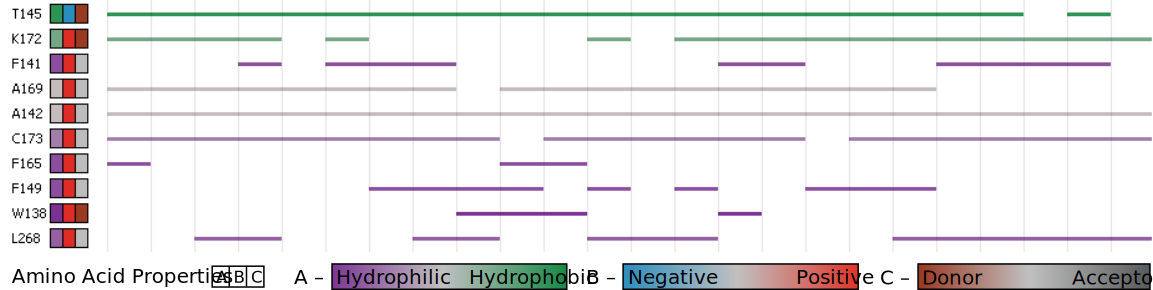
\includegraphics[width=0.95\linewidth]{img/aacids.png}
  \caption{\label{fig:aacids} Representation of amino acids surrounding the temporal tunnel and their physico-chemical properties. Coloring corresponds to a selected property, the line interruption means that this amino acid was not detected around the ligand in the corresponding temporal block.}
\end{figure}


\subsubsection*{Scatterplot Matrix}
For detailed analysis of geometrical and chemico-physical attributes of the ligand trajectory at given time steps, we propose Scatterplot Matrix.
The axes of one scatterplot represent a pair user-selected attributes.
Each point in the scatterplot then represents the values of these attributes at one time step.
As a result the scatterplot can easily reveal trends and relationships between attributes.
Interactive manipulation with scatterplot, such as selection, zooming and change of displayed attributes provides easy way of manual data filtering. 
To eliminate the noise in the data caused by ligand jittering, we propose several smoothing and aggregation functions.
\todo{nechat len sliding window?} 
The Sliding window function assigns to each time step averaged value of its neighborhood.
The size of the neighborhood is user regulated. 

The plots can further be stacked, forming a matrix and thus showing relationship between multiple attributes at once.
The stacked plots are also interactively interconnected.
The selection in Scatterplot Matrix is interactively linked with Barchart View.

\begin{figure}[htb]
	\centering
  \includegraphics[width=0.95\linewidth]{img/scatterplot.png}
  \caption{\label{fig:scatterplot} CHANGE!!! Scatterplot Matrix depicting Time vs. Distance and Time vs Speed property before (up) and after (down) smoothing by Sliding Window Function.}
\end{figure}


\subsection*{Analysis Procedure - BK, JP}

\section*{Results and Discussion - BK}
use case + feedback

\section*{Conclusions - All}
and future work 

%%%%%%%%%%%%%%%%%%%%%%%%%%%%%%%%%%%%%%%%%%%%%% 
%%                                          %%
%% Backmatter begins here                   %%
%%                                          %%
%%%%%%%%%%%%%%%%%%%%%%%%%%%%%%%%%%%%%%%%%%%%%%

\begin{backmatter}

\section*{Competing interests}
The authors declare that they have no competing interests.


%%%%%%%%%%%%%%%%%%%%%%%%%%%%%%%%%%%%%%%%%%%%%%%%%%%%%%%%%%%%%
%%                  The Bibliography                       %%
%%                                                         %%
%%  Bmc_mathpys.bst  will be used to                       %%
%%  create a .BBL file for submission.                     %%
%%  After submission of the .TEX file,                     %%
%%  you will be prompted to submit your .BBL file.         %%
%%                                                         %%
%%                                                         %%
%%  Note that the displayed Bibliography will not          %%
%%  necessarily be rendered by Latex exactly as specified  %%
%%  in the online Instructions for Authors.                %%
%%                                                         %%
%%%%%%%%%%%%%%%%%%%%%%%%%%%%%%%%%%%%%%%%%%%%%%%%%%%%%%%%%%%%%

% if your bibliography is in bibtex format, use those commands:
\bibliographystyle{bmc-mathphys} % Style BST file
\bibliography{bmc_article}      % Bibliography file (usually '*.bib' )

% or include bibliography directly:
% \begin{thebibliography}
% \bibitem{b1}
% \end{thebibliography}

%%%%%%%%%%%%%%%%%%%%%%%%%%%%%%%%%%%
%%                               %%
%% Figures                       %%
%%                               %%
%% NB: this is for captions and  %%
%% Titles. All graphics must be  %%
%% submitted separately and NOT  %%
%% included in the Tex document  %%
%%                               %%
%%%%%%%%%%%%%%%%%%%%%%%%%%%%%%%%%%%

%%
%% Do not use \listoffigures as most will included as separate files

%\section*{Figures}
%  \begin{figure}[h!]
 % \caption{\csentence{Sample figure title.}
  %    A short description of the figure content
   %   should go here.}
   %   \end{figure}

%\begin{figure}[h!]
 % \caption{\csentence{Sample figure title.}
  %    Figure legend text.}
  %    \end{figure}

%%%%%%%%%%%%%%%%%%%%%%%%%%%%%%%%%%%
%%                               %%
%% Tables                        %%
%%                               %%
%%%%%%%%%%%%%%%%%%%%%%%%%%%%%%%%%%%

%% Use of \listoftables is discouraged.
%%
%\section*{Tables}
%\begin{table}[h!]
%\caption{Sample table title. This is where the description of the table should go.}
 %     \begin{tabular}{cccc}
%        \hline
 %          & B1  &B2   & B3\\ \hline
 %       A1 & 0.1 & 0.2 & 0.3\\
 %       A2 & ... & ..  & .\\
 %       A3 & ..  & .   & .\\ \hline
 %     \end{tabular}
%\end{table}

%%%%%%%%%%%%%%%%%%%%%%%%%%%%%%%%%%%
%%                               %%
%% Additional Files              %%
%%                               %%
%%%%%%%%%%%%%%%%%%%%%%%%%%%%%%%%%%%

%\section*{Additional Files}
%  \subsection*{Additional file 1 --- Sample additional file title}
%    Additional file descriptions text (including details of how to
%    view the file, if it is in a non-standard format or the file extension).  This might
%    refer to a multi-page table or a figure.

%  \subsection*{Additional file 2 --- Sample additional file title}
%    Additional file descriptions text.

\end{backmatter}
\end{document}
